\subsubsection{Test \ref{test5}, BFS and DFS searches return correct values for a graph with one vertex.}
Input:  On a graph containing a single vertex A, click on the \enquote{Depth First Search} button, observe the message in the status bar, then click on the "Breadth First Search" button, and observe the message in the status bar.
\newline
\newline
Expected output: For the Depth First Search button, the status bar should display \enquote{DFS: A}, with no additional content. For the Breadth First Search button, the status bar should display \enquote{BFS: A} with no additional content.
\begin{figure}[ht]
    \centering
    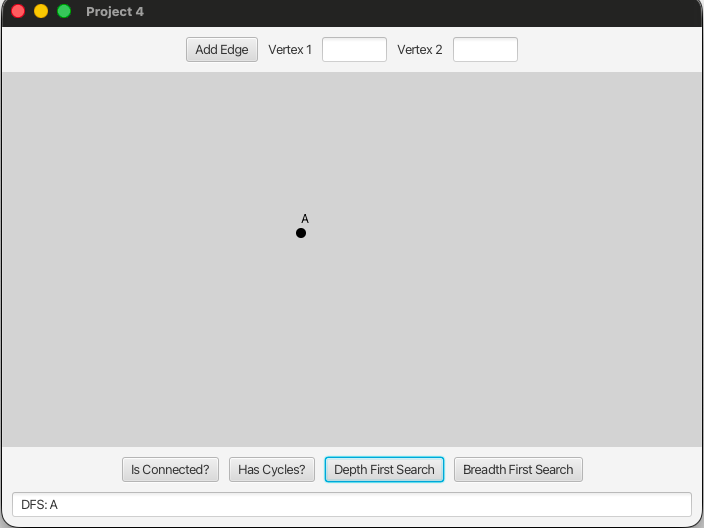
\includegraphics[width=0.65\textwidth]{images/test5-dfs.png}
    \caption{test \ref{test5} - Depth First Search button}
\end{figure}
\begin{figure}[ht]
    \centering
    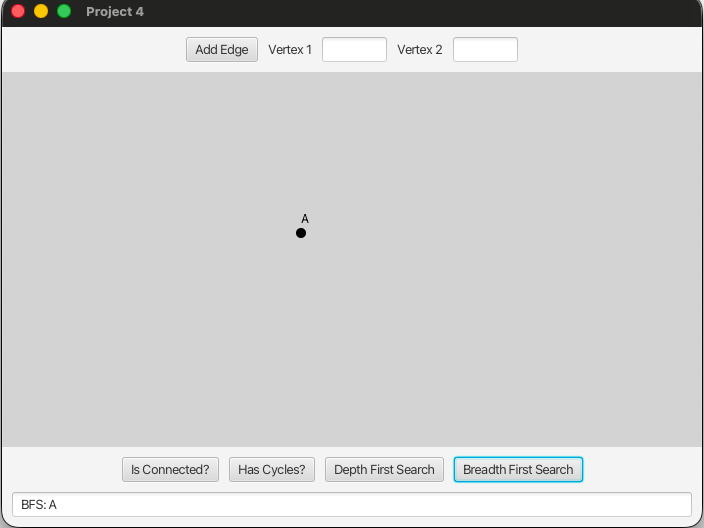
\includegraphics[width=0.65\textwidth]{images/test5-bfs.png}
    \caption{test \ref{test5} - Breadth First Search button}
\end{figure}
